% Generated by thesis/ch7/exp2/networks.py -- do not edit by hand.
\begin{sidewaysfigure}
  \centering
  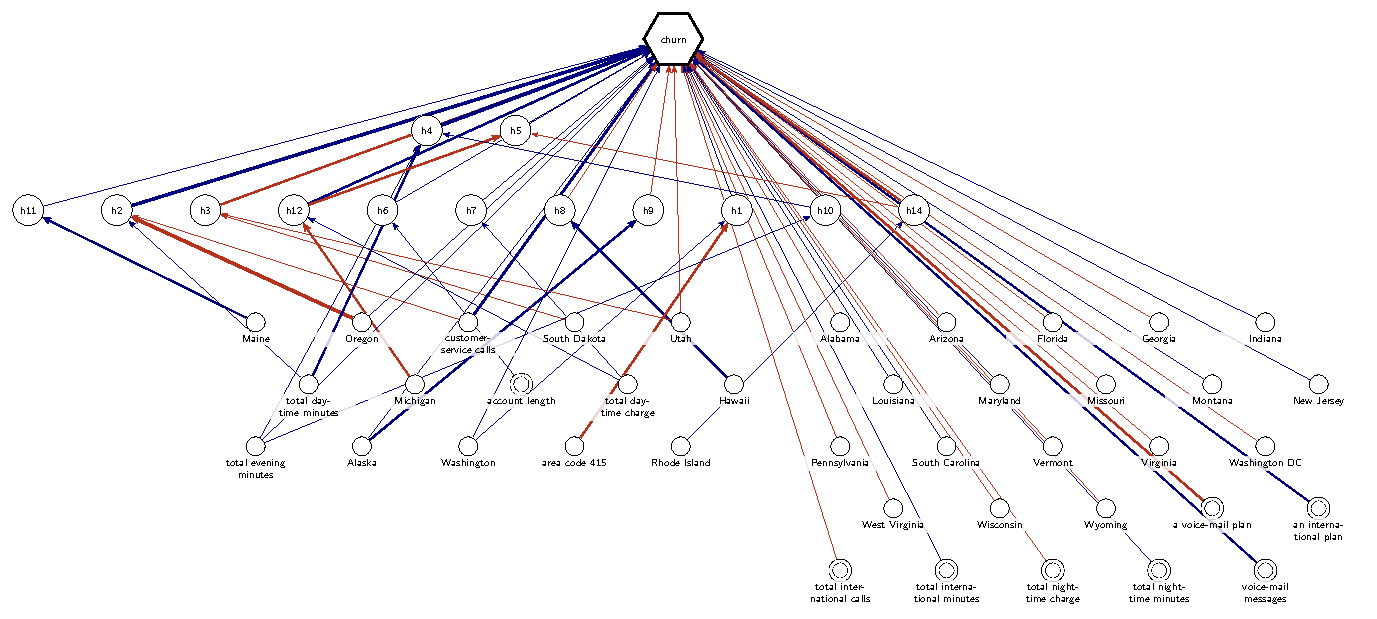
\includegraphics[width=\textheight,height=0.78\textwidth,keepaspectratio]{figures/exp2/networks/churn100-s4-raw}
  \caption{Churn, seed 4 (churn100-s4): the network as trained, before any explanation, in full. Inputs at the bottom (every input column its own node), hidden units by depth, the output at the top; 40 of 71 input columns are connected, with 13 hidden units and 64 enabled connections. Blue: positive weight (raises the score); red: negative weight (lowers it); thicker: larger weight. Orange outline and up arrow: raises the final prediction; teal and down arrow: lowers it; grey and double arrow: depends. Not used (no connection; 31 columns): Iowa, Idaho, Illinois, Kansas, Kentucky, Massachusetts, Arkansas, Minnesota, Mississippi, North Carolina, North Dakota, Nebraska, New Hampshire, New Mexico, Nevada, New York, Ohio, Oklahoma, California, Tennessee, Texas, Colorado, Connecticut, Delaware, area code 408, area code 510, total daytime calls, total evening calls, total evening charge, total night-time calls and total international charge.}
  \label{fig:exp2-net-churn100-s4-raw}
\end{sidewaysfigure}
